\section{Различные улучшения алгоритма Position Based Dynamics} \label{ch2:pbd-improvments} %название по-русски
	Алгоритм, описанный в предыдущей главе, позволяет симулировать поведение мягких тел, однако не может быть применен на практике. Поэтому. в статье \cite{pbd}, помимо основной идеи алгоритма, были предложены различные улучшения.
	
	Во-первых, симулируемое таким образом мягкое тело не взаимодействует с дургими физическими телами. Визуально это будет выглядеть как то, что оно будет \say{проходить сквозь} другие тела. Для того чтобы это обойти, используются алгоритмы обнаружения столкновений. В статье \cite{pbd} для решения этой проблемы предлагается динамически создавать новые ограничения с параметрами:
	\begin{enumerate}[1.]
		\item Функцию $C(p^*) = (p^* - q) * n$, где $q$ - точка пересечения луча (выходящего из положения частицы $p$ в направлении предсказанного положения частицы $p^*$) с поверхностью твердого объекта, а $n$ - вектор нормали в точке $q$
		\item Параметр жесткости $k = 1$
		\item тип \say{неравенства}
	\end{enumerate}
	Таким образом получается достичь \say{одностороннего взаимодействия} - мягкое тело отткалкивается от твердых, но твердые тела не получают импульсов от мягких. Чтобы добиться \say{двухстороннего взаимодействия}, авторами было принято решения применять импульс равный $\frac{m_i*(p_i(t + \delta t) - p_i(t))}{\delta t}$ за каждую частицу, для которой сработало сгенерированное ограничение описанное ранее.
		
	Во-вторых, симулирумое мягкое тело не взаимодействует с частями самого же себя. Т.е. если частицы не соединены ограничениями напрямую, то эти чатицы могут свободно перемещаться друг относительно друга, что приводит к самопересечениям. В статье \cite{pbd} авторы предлагают разбить поверхность мягкого тела на треугольники и проверять пересечение частиц с треугольниками заданными тремя вершинами $p_1^t, p_2^t, p_3^t$ и толщиной $h$ при помощи функций:
	\begin{equation}
		C(p^*, p_1^t, p_2^t, p_3^t) = (p^* - p_1^t) \cdot \frac{(p_2^t - p_1^t) \times (p_3^t - p_1^t)}{|(p_2^t - p_1^t) \times (p_3^t - p_1^t)|} - h
	\end{equation}
	Или, если частица входит в треугольник со стороны обратной стороне нормали
	\begin{equation}
		C(p^*, p_1^t, p_2^t, p_3^t) = (p^* - p_1^t) \cdot \frac{(p_3^t - p_1^t) \times (p_2^t - p_1^t)}{|(p_3^t - p_1^t) \times (p_2^t - p_1^t)|} - h
	\end{equation}	
	Таким образом возможно избавиться от самопересечений, однако если просто проверять все возможные частицы со всеми возможными треугольниками, данный алгоритм окажется излише нагруженным с точки зрения времени выполнения. Для того чтобы отсечь часть проверяемых треугольников, авторами используется алгоритм пространственного хеширования треугольников описанный в \cite{teschner2003optimized}.
	
	В-третьих, для удаления колебаний, авторы используют демпферирование, уменьшая скорости (полученные на этапе предсказания положений частиц) используя константу демпферирования. Таким образом, результирующий алгоритм выглядит так, как показано на \firef{alg:PositionBasedDynamics2}.
	
	\begin{algorithm} %[h]
		\SetKwFunction{algoPBDTwoPseudocode}{} 
		\SetKwProg{myalg}{Algorithm}{}{} %write in 2nd agrument <<Algorithm>>, <<Procedure>> etc
		\nonl\myalg{\algoPBDTwoPseudocode}{
			\KwInput{
				время шага симуляции $\delta t$,
				количество итераций $solverIteration$,
				текущее состояние частиц,
				предыдущее состояние частиц,
				ограничения,
				функция суммы внешних сил от положения $f_{ext}(p)$,
			}
			\KwOutput{положение частиц спустя заданное время $p_i(t + \delta t)$}
			
			\For {$\forall p_i $\label{step:pbd-solver-integrate-vel}}{
				$v_i \leftarrow \frac{p_i(t) - p_i(t -\delta t)}{\delta t} + \delta t * im_i * f_{ext}(p_i)$;
			}
			
			$dampVelocities(v_1, ... v_N)$
			
			\For {$\forall p_i $\label{step:pbd-solver-integrate-pos}}{
				$p^*_i \leftarrow p_i(t) + v_i * \delta t $;
			}

			\For {$\forall p_i $\label{step:pbd-solver-collision}}{
				$generateCollisionConstraints(p_i -> p^*_i)$;
			}
			
			\For{$\forall k \in 1..solverIteration$  \label{step:pbd-solver-loop}}{
				$p^*_1, ..., p^*_N \leftarrow projectConstraints(p^*_1, ..., p^*_N)$;
			}
			
			\For {$\forall p_i $\label{step:pbd-solver-save}}{
				$p_i(t + \delta t) \leftarrow p^*_i$\;
			}
		}
		\caption{Псевдокод алгоритма Position Based Dynamics с учетом коллизий и демпферирования}\label{alg:PositionBasedDynamics2}
	\end{algorithm}
	\FloatBarrier
	
	Как можно заметить, сложность данного алгоритма пропорциональна произведению числа частиц на число итераций. В связи с этим, авторы многих статей ставили перед собой цель уменьшить два этих параметра, при это сохраняя точность.
	
	Так в статье \cite{muller2010wrinkle} авторами было замечено, что при увеличении размерности сетки, основной добавляемой деталью являются небольшие складки, не сильно влияющие на глобальное поведение ткани. Тогда было решено разделить ткань на глобальную сетку с низким числом частиц, и локальную сетку с высоким числом частиц. Основной алгоритм симуляции ткани (вместе с обработкой пересечений) производился на глобальной сетке. Тем временем локальная сетка прикреплялась к глобальной сетке и не требовала большого количества итераций(\firef{fig:wrincle-idea} и \firef{fig:wrincle-show}).
	\newpage
	
	\begin{figure}[ht!] 
		\center
		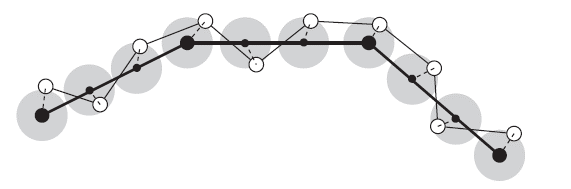
\includegraphics [scale=1] {my_folder/images//wrincle_mesh_idea}
		\caption{Схема идеи алгоритма складок. Черные точки - вершины глобальной сетки, белые точки - вершины локальной сетки. Прикрепление локальной сетки к глобальной происходит за счет добавления ограничений на расстояние, представленых в виде серых дисков}
		\label{fig:wrincle-idea}  
	\end{figure}
	
		
	\begin{figure}[ht!] 
		\center
		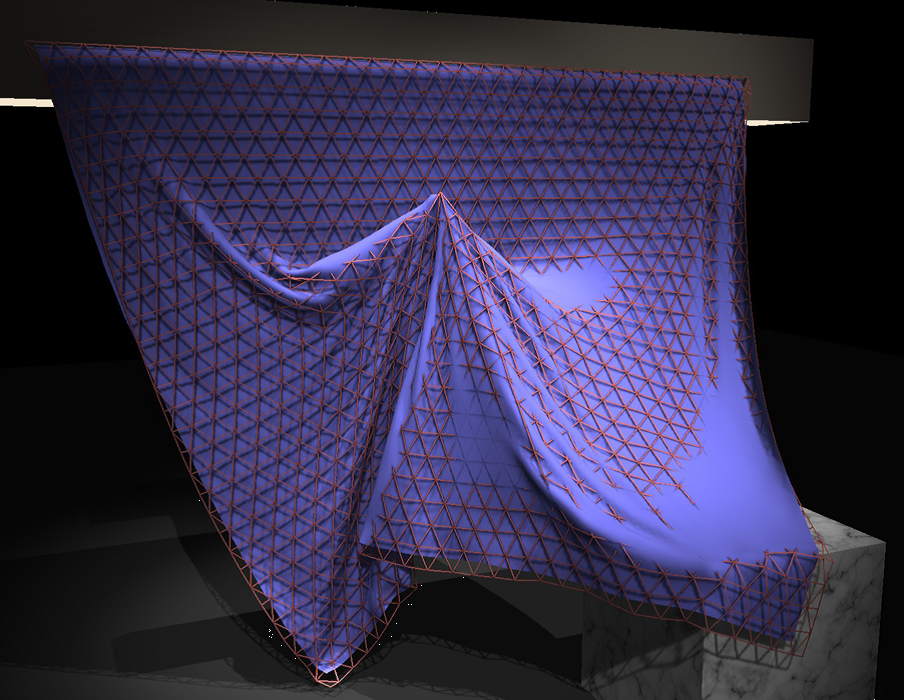
\includegraphics [scale=0.7] {my_folder/images//wrincle_mesh_show}
		\caption{Визуальная демонстрация алгоритма складок. Красным представлена глобальная сетка, а фиолетоым представлена ткань локальной сетки}
		\label{fig:wrincle-show}  
	\end{figure}
	
	А другой статье \cite{kim2012long} авторами была предпринята попытка решить проблему глобального растяжения ткани, в случае малого числа итераций. Для этого они разработали технику Long Range Attachments. Она основывается на том, что зачастую растяжение ткани проявляется в ситуациях, когда ткань закреплена какими-то частицами. Идея данной техники заключается в том, чтобы связывать ограничениями не только вершину с соседними вершинами, а также создать ограничения, соедниняющее закрпеленную вершину с другими вершинами таким образом, чтобы другие вершины не могли растянуться (\firef{fig:lra}).
	
	\begin{figure}[ht!] 
		\center
		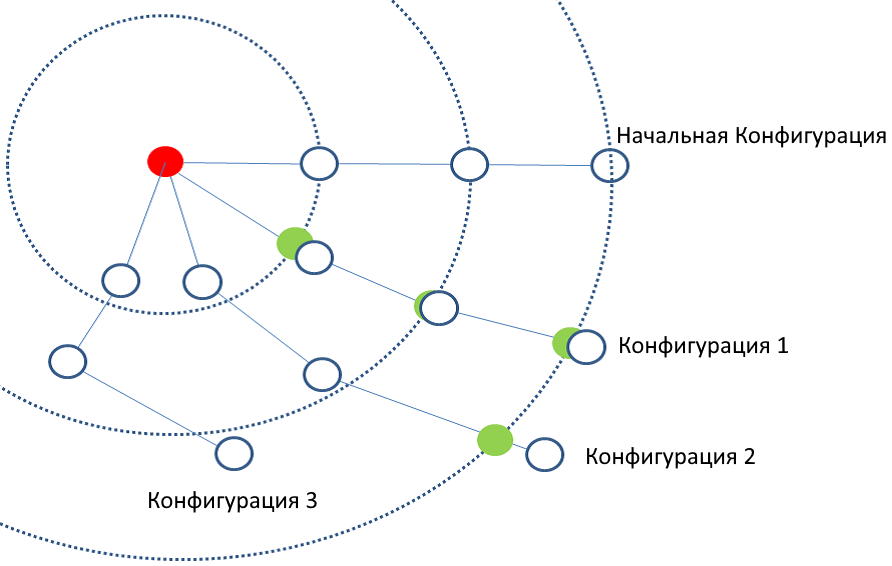
\includegraphics [scale=0.9] {my_folder/images//lra}
		\caption{Схема идеи алгоритма Long Range Attachments на примере нерастяжимой веревки. Красным цветом обозначена закрепленная вершина. Каждая другая вершина удерживается или остается внутри соответствующей ей сферы (представленной пунктиром). Для каждой конфигурации (если вершина оказалась за пределами своей сферы) зеленым представлено положение, исправленное алгоритмом LRA}
		\label{fig:lra}  
	\end{figure}
	
	Наконец, возникает вопрос как именно задавать различные мягкие тела при помощи ограничений. Данная работа посвещена симуляции тканей, поэтому решается вопрос относительно их. В современных системах симуляции тканей используется два основных подхода: через задание прямоугольной сетки и через использование триангулированной геометрии.
	
	Для первого случая, используются следующие ограничения	
	\begin{enumerate}[1.]
		\item Ограничение растяжения/структурное ограничение (Structural/streching). Определяется как растяжение типа \say{пружина}, соединяющее соседние ячейки как показано на \firef{fig:structural}. Задает структуру всей ткани
		\item Ограничение сдвига (Shear). Определяется как растяжения типа \say{пружина} соединяющее диагональные ячейки как показано на \firef{fig:shear}. Помогает в ситуации представленной на \firef{fig:shear_blender}.
		\item Ограничение изгиба (Bending). Может определяться как ограничение на угол \cite{wang2014angle}, а может как ограничение типа \say{пружина}, соединяющее ячейки \say{через одну} как показано на \firef{fig:bending}.
	\end{enumerate}
	
	\begin{figure}[ht!] 
		\center
		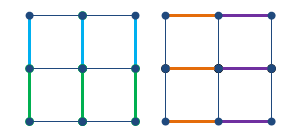
\includegraphics [scale=0.5] {my_folder/images//structural}
		\caption{Визуальная демонстрация структурных ограничений}
		\label{fig:structural}  
	\end{figure}
	
	\begin{figure}[ht!] 
		\center
		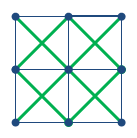
\includegraphics [scale=0.5] {my_folder/images//shear}
		\caption{Визуальная демонстрация ограничений сдвига}
		\label{fig:shear}  
	\end{figure}
	
	\begin{figure}[ht!] 
		\center
		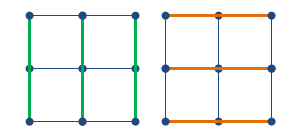
\includegraphics [scale=0.5] {my_folder/images//bending}
		\caption{Визуальная демонстрация ограничений изгиба}
		\label{fig:bending}  
	\end{figure}
	
	\begin{figure}[ht!] 
		\center
		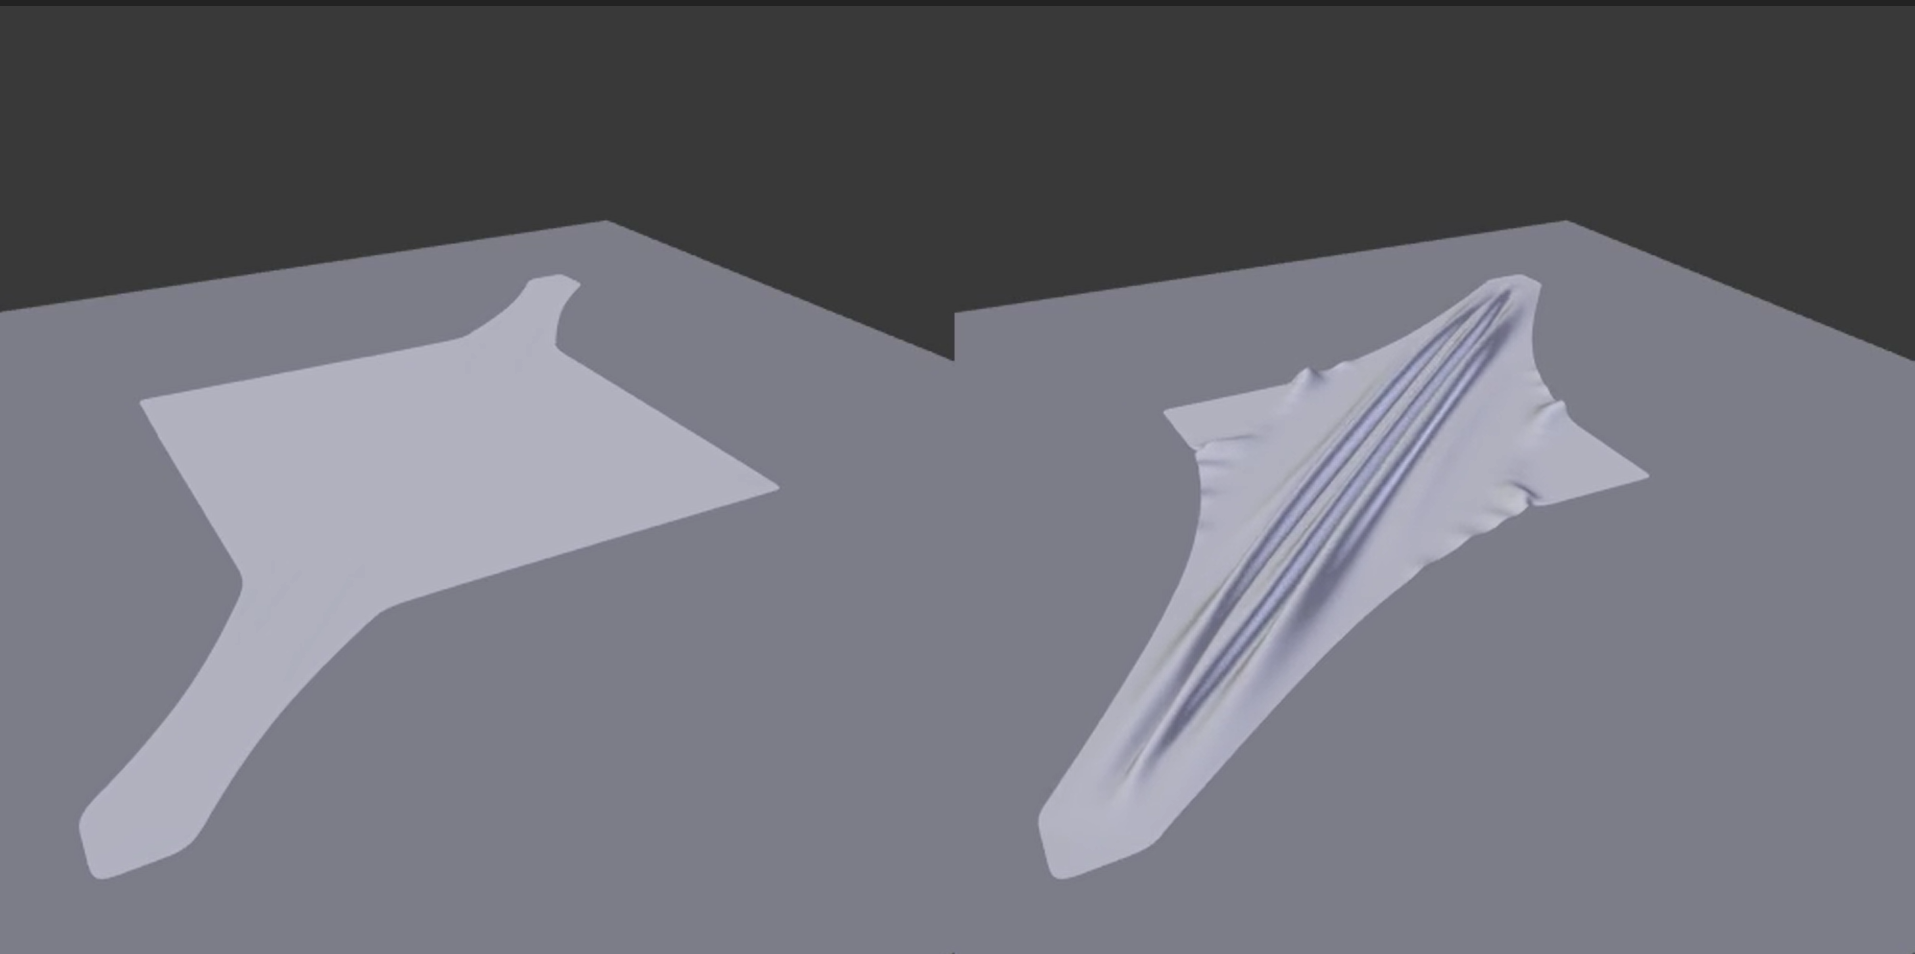
\includegraphics [scale=0.2] {my_folder/images//shear_blender}
		\caption{Сравнение тканей с отсутствием ограничения сдвига (слева) и наличием ограничения сдвига (справа)}
		\label{fig:shear_blender}  
	\end{figure}

	Во втором случае, имеющаяся триангулированная геометрия проходит через предобработку, в которой вышеописанные ограничения (для прямоугольной сетки) накладываются на вершины триангулированной геометрии. Для этого триангулированная геометрия разбивается на прямоугольные сетки (для которых ограничения известны), а затем эти прямоугольные сетки \say{сшиваются} между собой используя структурные ограничения.
	
%% Вспомогательные команды - Additional commands
%
%\newpage % принудительное начало с новой страницы, использовать только в конце раздела
%\clearpage % осуществляется пакетом <<placeins>> в пределах секций
%\newpage\leavevmode\thispagestyle{empty}\newpage % 100 % начало новой страницы